%   PACKAGES AND CUSTOMIzATIONS  %%%%%%%%%%%%%%%%%%%%%%%%
\documentclass[12pt]{article}
\usepackage{amsmath}
\usepackage{amssymb}
\usepackage{amsthm}
\usepackage[pdfborder={0 0 0}]{hyperref}
\usepackage{graphicx}
\usepackage{caption}
\usepackage{natbib}
\usepackage{wrapfig}
\usepackage{enumitem}
\setlist[enumerate]{itemsep=0mm}
\usepackage{multirow}
\usepackage{lscape}
\usepackage{caption}
\usepackage{subcaption}
\usepackage{float}
\usepackage{hyperref}
\usepackage{tabularx}
\usepackage{rotating}
\captionsetup[subfigure]{position=top, labelfont=bf,textfont=normalfont,singlelinecheck=off,justification=raggedright}
\renewcommand{\vector}[1]{\mathbf{#1}}
\usepackage{adjustbox}
\usepackage{bm}
\usepackage{booktabs}



\newcommand{\transectAbb}{Data for each glacier are divided into lower hourglass (LH), lower circle (LC), lower midline (LM), upper hourglass (UH), upper circle (UC), upper midline (UM), and upper transect (UT).}
\newcommand{\params}{Topographic parameters are distance from centreline ($d_C$), elevation ($z$), aspect ($\alpha$), slope ($m$), northness ($N$), curvature ($\kappa$), and Sx. }
\newcommand{\boxplot}{Within each box, the mean is shown as a circle, the median as a horizontal line, the interquartile range (IQR) as a coloured box, two times the IQR as dashed lines beyond the box, and outliers as single points. }
\newcommand{\boxMatlab}{Red line indicates median, blue box shows first quantiles, bars indicate minimum and maximum values (excluding outliers), and red crosses show outliers, which are defined as being outside of the range of 1.5 times the quartiles (approximately $\pm2.7\sigma$). }
\newcommand{\topomap}{Arrows indicate glacier flow direction and black dots show snow depth sampling locations. }
\newcommand{\swedots}{Observed SWE values are overlain on the maps. }


\begin{document}

\section{Winter Surface Mass Balance Distribution}
\label{sec:WSMBdistribution}

\subsection{Background}

We identify three major sources of variability within the process of translating snow measurements to winter surface mass balance (WSMB). These variability sources encompass error and uncertainty within each processing step. We refer to the three variability sources as (1) density variability, (2) SWE variability and (3) interpolation variability. To quantify the effects of these sources of variability, a Monte Carlo sampling of the distribution of SWE variability and interpolation variability is used to obtain a distribution of WSMB for eight chosen density interpolation methods.  

\subsection{Methods}

To quantify the effects of the three variability sources on the final WSMB estimate, we conduct a Monte Carlo experiment, which uses repeated random sampling to calculate a numerical solution \citep{Metropolis1949}. In our study, we randomly sample the distributions for SWE variability and interpolation variability and carry these values through the data processing steps to obtain a value of WSMB. First, random values from the distribution of SWE values for each grid cell are independently chosen. Then, LR or SK is used to interpolate these SWE values. With the LR, a set of $\beta_i$ values and their distributions are calculated and the $\beta_i$ distributions are randomly sampled. These new $\beta_i$ values are used to calculate WSMB. With SK, a distribution of WSMB is calculated from the 95\% confidence interval kriging surfaces. Density variability is accounted for by repeating the process for each density interpolation method. This random sampling process is done 1000 times, which results in a distribution of possible WSMB values based on variability within the data processing steps.


\subsubsection{SWE variability}

Variability in observed SWE is included by generating a normal distribution with $\mu=0$ and a standard deviation equal to the glacier-wide mean standard deviation of the observed zigzag SWE values ($\sigma_{\mathrm{G4}} = 0.027 $ m w.e., $\sigma_{\mathrm{G2}} = 0.035$ m w.e., $\sigma_{\mathrm{G13}} = 0.040 $ m w.e.). A random set of values is drawn from this distribution and added to the SWE values used to calculate the regression. SWE values that end up being less than zero are assigned a SWE of zero.

\subsubsection{Interpolation variability}

For the linear regression, variability from regression coefficient estimation was found by first calculating linear regression coefficients ($\boldsymbol{\beta}$) using cross-correlation and BIC weighting of multivariate linear regression models (Section \ref{sec:MLR}). A set of multivariate normal random regression coefficient distributions are then found using the coefficient covariance and coefficient values from the linear regression using the built-in function \texttt{mvnrnd}. The covariance of regression coefficients is given by \citep{Bagos2015}:
\begin{equation}
\mathrm{cov}\left( \boldsymbol{\beta} \right) = \sigma^2 \left( \boldsymbol{X}'  \boldsymbol{X} \right)^{-1}
\end{equation}
where $\boldsymbol{X}$ is the $n \times k$ matrix of predictor variables. The variance of the regression, $\sigma^2$, is estimated using
\begin{equation}
\sigma^2 = \frac{\sum^n_{i=1} \left(\boldsymbol{y}_i-\bar{\boldsymbol{y}} \right)^2}{n-k-1}
\end{equation}
The distributions of each $\beta$ are sampled 1000 times and the WSMB is calculated for each set of coefficients.

Simple kriging (SK) variability is calculated using the DiceKriging package. The upper and lower 95\% confidence interval (CI) for SWE at each grid cell are returned and the mean WSMB for the upper and lower limits is then calculated. When there is no SWE variability then the SK variability is assumed to be normally distributed between the upper and lower CI. When SWE variability is introduced, upper and lower CI values are calculated for each SWE variability random sampling. The mean upper and lower CIs are then used to find a normal distribution for SK variability combined with SWE variability. 

\subsection{Results}

\subsubsection{WSMB uncertainty}

Specific WSMB is affected by variability introduced when interpolating density (density variability), when calculating grid cell SWE values (SWE variability), and when interpolating observations (interpolation variability). We find that when using a LR, interpolation variability has a larger effect on WSMB uncertainty than density variability or SWE variability. The probability density function (PDF) that arises from SWE variability is much narrower than the PDF that arises from interpolation variability (Figure \ref{fig:WSMBDist_LR} and Table \ref{tab:WSMBdistribution_sigma}). WSMB uncertainty found with SK interpolation is dominated by interpolation variability (Table \ref{tab:WSMBdistribution_sigma}).  

 \begin{table}[]
\centering
\caption{Standard deviation ([m w.e.]) of specific winter surface mass balance estimated using linear regression (LR) and simple kriging (SK) when variability is introduced. Density variability ($\sigma_{\rho}$) is the standard deviation of WSMB estimated using SWE data with different density interpolation methods. SWE variability ($\sigma_{\mathrm{SWE}}$) is approximated by a normal distribution about the local SWE value with standard deviation equal to the glacier-wide mean zigzag standard deviation. LR interpolation variability ($\sigma_{\beta}$) is accounted for by varying the regression coefficients with a normal distribution with standard deviation calculated from regression covariance. SK interpolation variability ($\sigma_{\mathrm{KRIG}}$) is taken from the range of distributed SWE estimates calculated by the DiceKriging package. Result for Glacier 4 (G4), Glacier 2 (G2) and Glacier 13 (G13) are shown.}
\label{tab:WSMBdistribution_sigma}
\begin{tabular}{ccccccc}
\textbf{} & \multicolumn{3}{c}{\textbf{Linear Regression}} & \multicolumn{3}{c}{\textbf{Simple Kriging}} \\
 & $\sigma_{\rho}$ & $\sigma_{\mathrm{SWE}}$ & $\sigma_{\beta}$ & $\sigma_{\rho}$ & $\sigma_{\mathrm{SWE}}$ & $\sigma_{\mathrm{KRIG}}$ \\
\midrule
\textbf{G4} & 0.0190 & 0.0086 & 0.0213 & 0.0215 & 0.0085 & 0.1405 \\
\textbf{G2} & 0.0337 & 0.0180 & 0.0309 & 0.0203 & 0.0253 & 0.1378 \\
\textbf{G13} & 0.0168 & 0.0112 & 0.0280 & 0.0127 & 0.0115 & 0.0965
\end{tabular}
\end{table}

\begin{figure*}
	\centering
\hspace*{-1.2cm}
	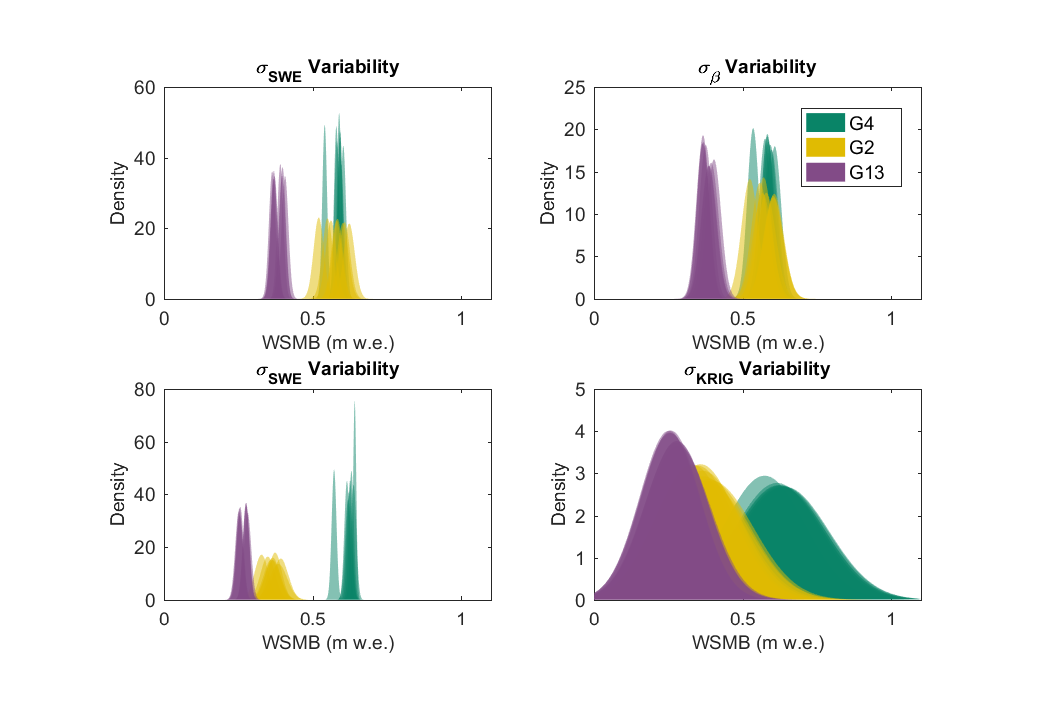
\includegraphics[width =1.2\textwidth]{WSMBDist_LR.pdf}\\
	\caption{Probability density functions (PDFs) fitted to distributions of specific winter surface mass balance (WSMB) values that arise from SWE variability ($\sigma_{ZZ}$) and interpolation variability ($\sigma_{\beta}$ or $\sigma_{\mathrm{KRIG}}$). Results from a linear regression interpolation (top panels) and simple kriging (bottom panels) are shown. Each PDF is calculated using one of eight density interpolation methods for Glacier 4 (G4), Glacier 2 (G2) and Glacier 13 (G13).}
	\label{fig:WSMBDist_LR}
\end{figure*}

The total WSMB uncertainty from SK interpolation is 3 to 5 times greater than uncertainty from LR interpolation. The PDFs overlap between the two interpolation methods although the PDF peaks are lower when SK is used for Glaciers 2 and 13 and higher for Glacier 4. SK results in WSMB distributions that overlap between glaciers and there is also a small probability of estimating a WSMB value of 0 m w.e. for Glaciers 2 and 13. LR results in overlapping WSMB distributions for Glaciers 2 and 4, with the PDF peak of Glacier 4 being slightly higher than that of Glacier 2. 

\begin{figure}
	\centering
	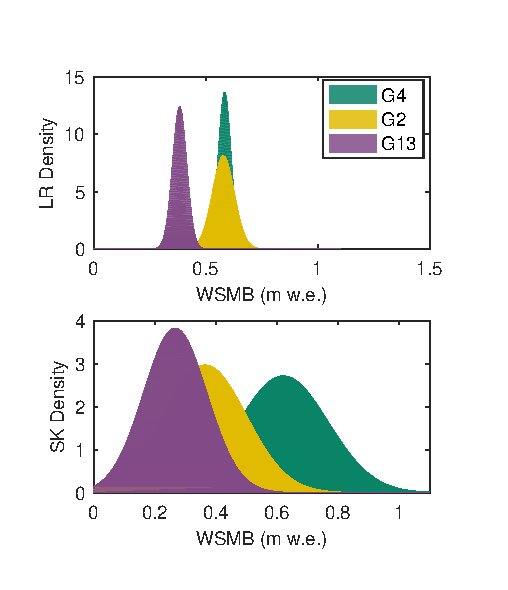
\includegraphics[width =0.8\textwidth]{WSMBDist_full.pdf}\\
	\caption{Probability density functions (PDFs) fitted to distributions of specific winter surface mass balance (WSMB) values estimated using linear regression (top) or simple kriging (bottom). Each PDF includes density variability, SWE variability and interpolation variability for Glacier 4 (G4), Glacier 2 (G2) and Glacier 13 (G13).}
	\label{fig:WSMBDist_LRvsSK}
\end{figure}


\subsubsection{Spatial patterns of winter balance uncertainty}

The spatial patterns of WSMB uncertainty are affected by density, SWE, and interpolation variability (Figure \ref{fig:WSMBspatialvar}).  For both LR and SK, the greatest variability in estimated SWE occurs in the accumulation area. When LR is used, estimated SWE is highly sensitive to the elevation regression parameter. In the case of SK, variability is greatest in areas far from observed SWE, which consist of the upper accumulation area on Glaciers 2 and 13. Variability is greatest on Glacier 4 when LR interpolation is used at the upper edges of the accumulation area, which correspond to the locations with extreme values of the wind redistribution parameter. When SK is used for interpolation on Glacier 4, variability is greatest at the measured grid cells, which highlights the short correlation length and the large effect of density interpolation on the SK accumulation estimate.

\begin{figure*}
	\centering
	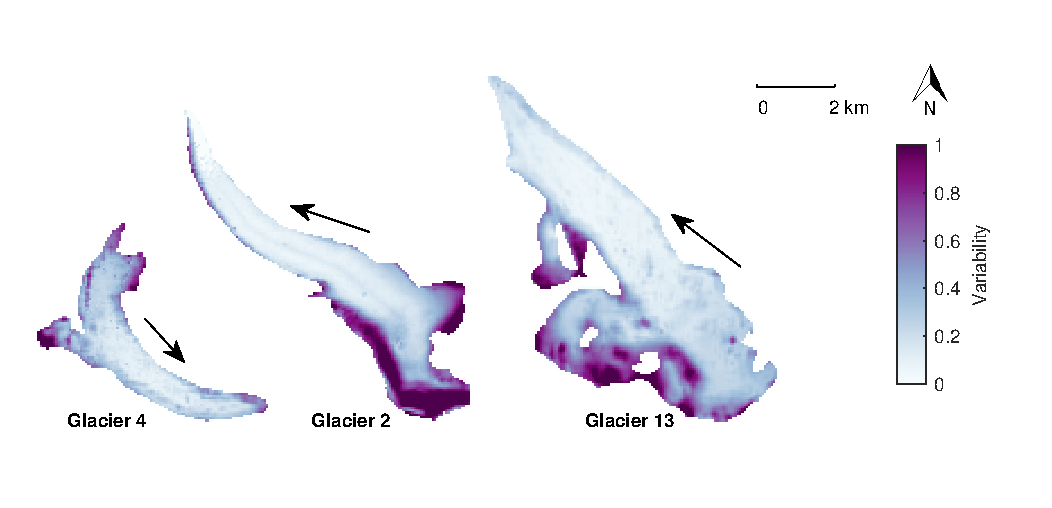
\includegraphics[width =\textwidth]{SpatialVar_LR.pdf}\\
	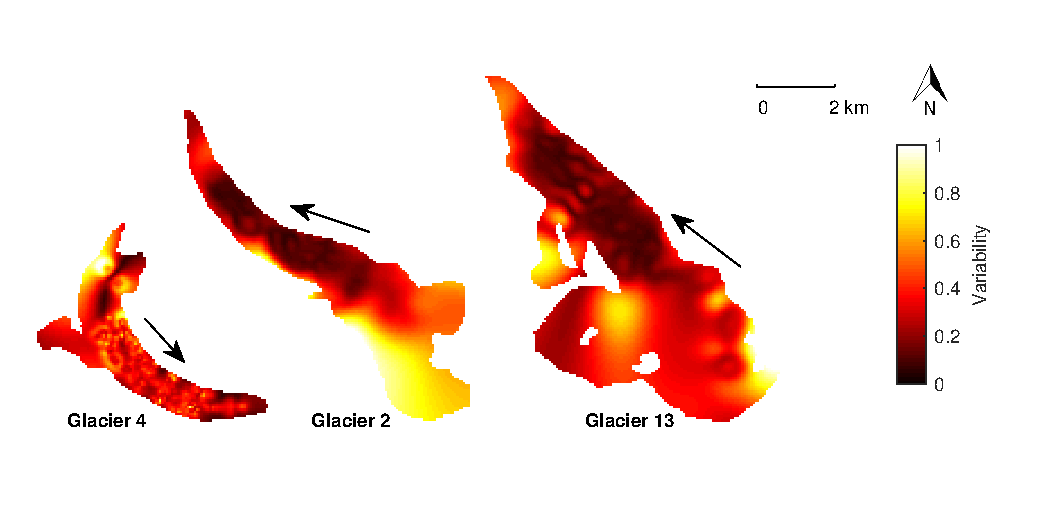
\includegraphics[width =\textwidth]{SpatialVar_SK.pdf}\\
	\caption{Variability of SWE estimated using linear regression (top) and simple kriging (bottom).	Variability is a relative quantity measured by taking the sum of differences between one hundred estimates of distributed WSMB that include SWE variability and, in the case of linear regression, regression variability. The sum is then normalized for each glacier. Glacier flow directions are indicated by arrows.}
	\label{fig:WSMBspatialvar}
\end{figure*}


\subsection{Discussion}

Interpolation variability is the greatest contributor to WSMB uncertainty for both SK and LR. This uncertainty arises from extrapolation beyond the sampled region, which results in highly variability in estimated SWE in the accumulation area. To reduce WSMB uncertainty, emphasis must therefore be placed on sampling in the accumulation area and generally obtaining measurements throughout the study basin. 

SWE variability is the smallest contributor to WSMB uncertainty. Therefore, obtaining the most accurate value of SWE to represent a grid cell, even a relatively large grid cell, does not need to be a priority when designing a snow survey. Extensively measuring SWE variability in a few locations using a zigzag design appears to be a good constraint on SWE variability. Many parts of a glacier though are characterized by a relatively smooth surface, with roughness lengths on the order of centimeters \citep{Hock2005} resulting in low snow depth variability. However, we assume that the sampled grid cells are representative of the variability across the entire glacier, which is likely not true for areas with debris cover, crevasses and steep slopes. Snow depth variability can be large and thus exert a dominant control on snow distribution in these area \citep{McGrath2015}. Effects of SWE variability in either smaller or larger grid cells could also be different so further investigation is needed.

Using a Monte Carlo experiment to propagate variability allowed us to quantify effects of variability on estimates of WSMB. However, our analysis did not include variability arising from a number of data sources. Error associated with SP and FS density measurement is not included but we believe that this error is likely to be encompassed in the wide range of density interpolation methods. DEM vertical and horizontal error are not considered in the Monte Carlo experiment mainly because there is no DEM validation data at our study location. Error associated with estimating measurement locations, which is a combination of hand-held GPS error, distance of observers from GPS and travel along a straight line, is also not considered. However, we feel that this source of error is encompassed in the variability estimated from zigzag measurements. 

%%%%%%%%%%%%%%%%%%%%%
\bibliography{/home/glaciology1/Documents/MastersDocuments/MastersLit}
\bibliographystyle{igs}
%%%%%%%%%%%%%%%%%%%%%

\section{APPENDIX}

\subsection{Linear regression WSMB distribution}

\begin{figure}[H]
	\centering
	\makebox[\textwidth][c]{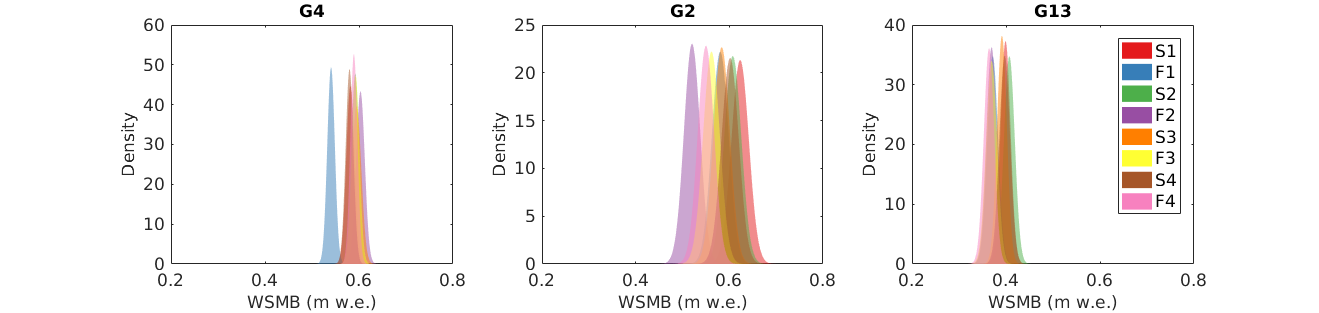
\includegraphics[width=1.2\textwidth]{WSMB_allDensity_zz.png}}\\%
	\makebox[\textwidth][c]{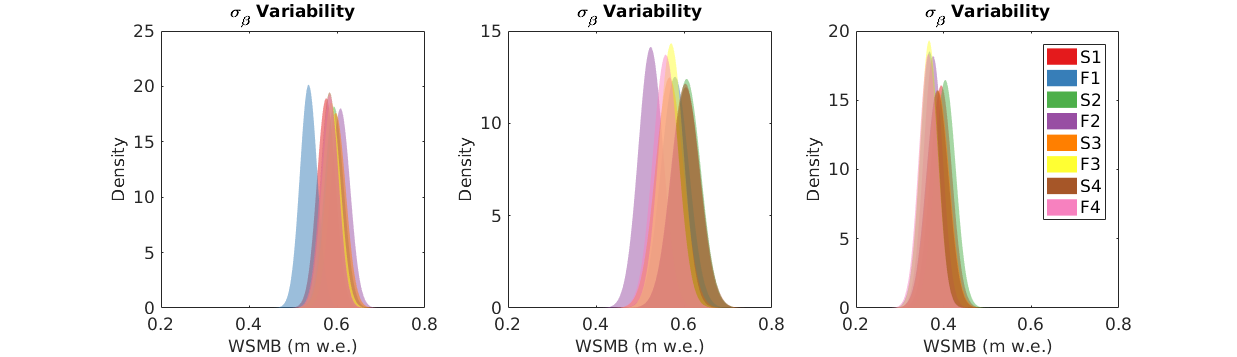
\includegraphics[width=1.2\textwidth]{WSMB_allDensity_beta.png}}\\%
	\makebox[\textwidth][c]{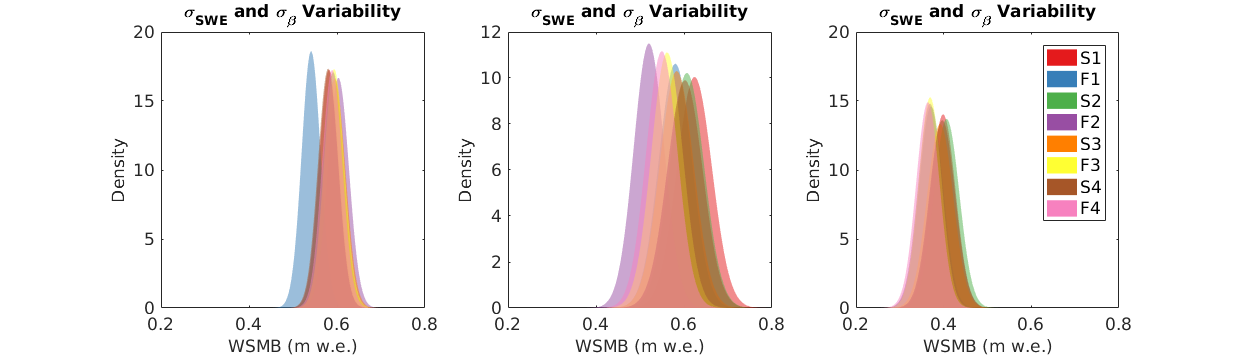
\includegraphics[width=1.2\textwidth]{WSMB_allDensity_betaNzz.png}}%
	\caption{Distribution of winter surface mass balance (WSMB) obtained using linear regression. (Top) WSMB values obtained from a Monte Carlo sampling of normally distributed SWE variation (obtained from zigzag measurements) about the local SWE value. (Middle) WSMB values obtained from a Monte Carlo sampling of normally distributed regression coefficients. (Bottom) WSMB values obtained using both SWE variability and regression coefficient variability. Eight different density interpolation methods are used to obtain SWE values used in the regression.}
	\label{fig:WSMB_allDensity}
\end{figure}


\begin{figure}[H]
	\centering
	\makebox[\textwidth][c]{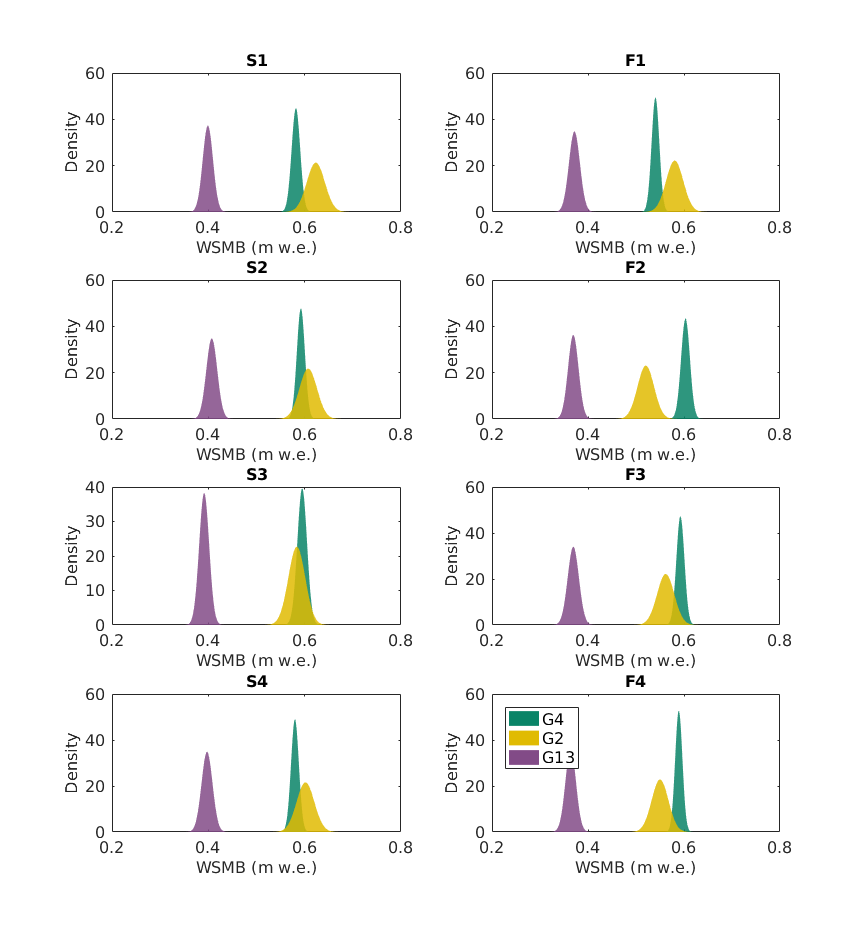
\includegraphics[width =1.2\textwidth]{WSMB_Distributionzz.png}}\\
	\caption{Winter surface mass balance distribution obtained using linear regression for eight density interpolation options when variation due to SWE measurement ( $\sigma_{ZZ}$) is included. }
	\label{fig:WSMB_Distributionzz}
\end{figure}
\begin{figure}[H]
	\centering
	\makebox[\textwidth][c]{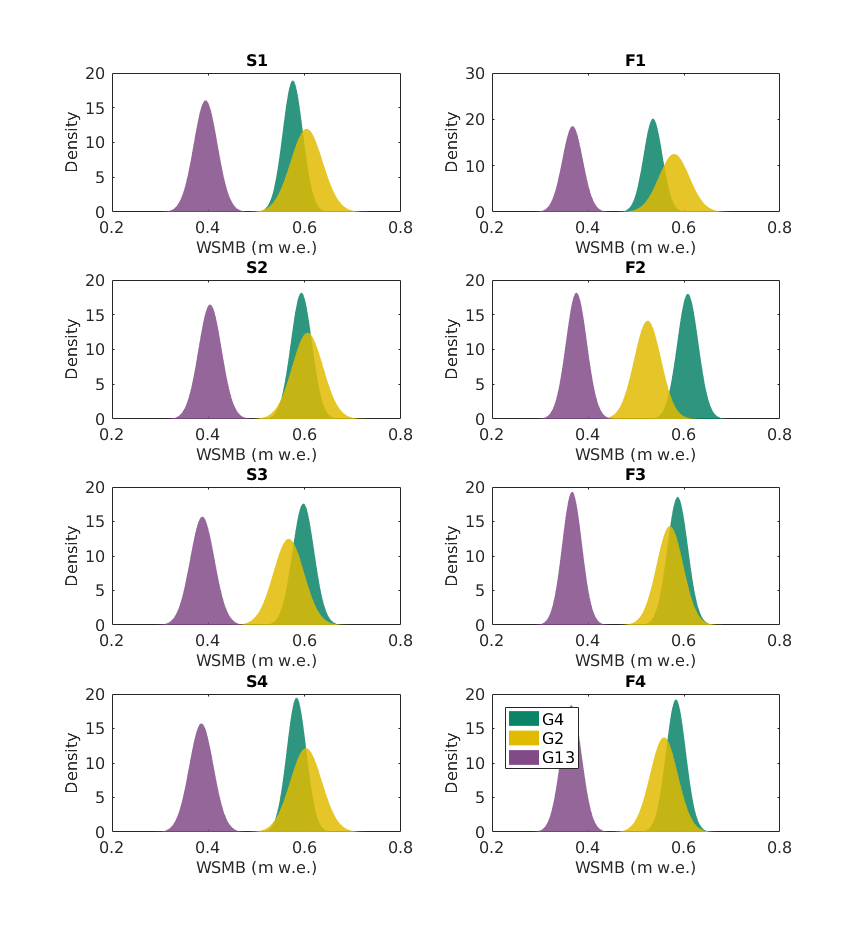
\includegraphics[width =1.2\textwidth]{WSMB_Distributionbeta.png}}\\
	\caption{Winter surface mass balance distribution obtained using linear regression for eight density interpolation options when variation due to regression coefficient estimation ( $\beta$) is included. }
	\label{fig:WSMB_Distributionbeta}
\end{figure}
\begin{figure}[H]
	\centering
	\makebox[\textwidth][c]{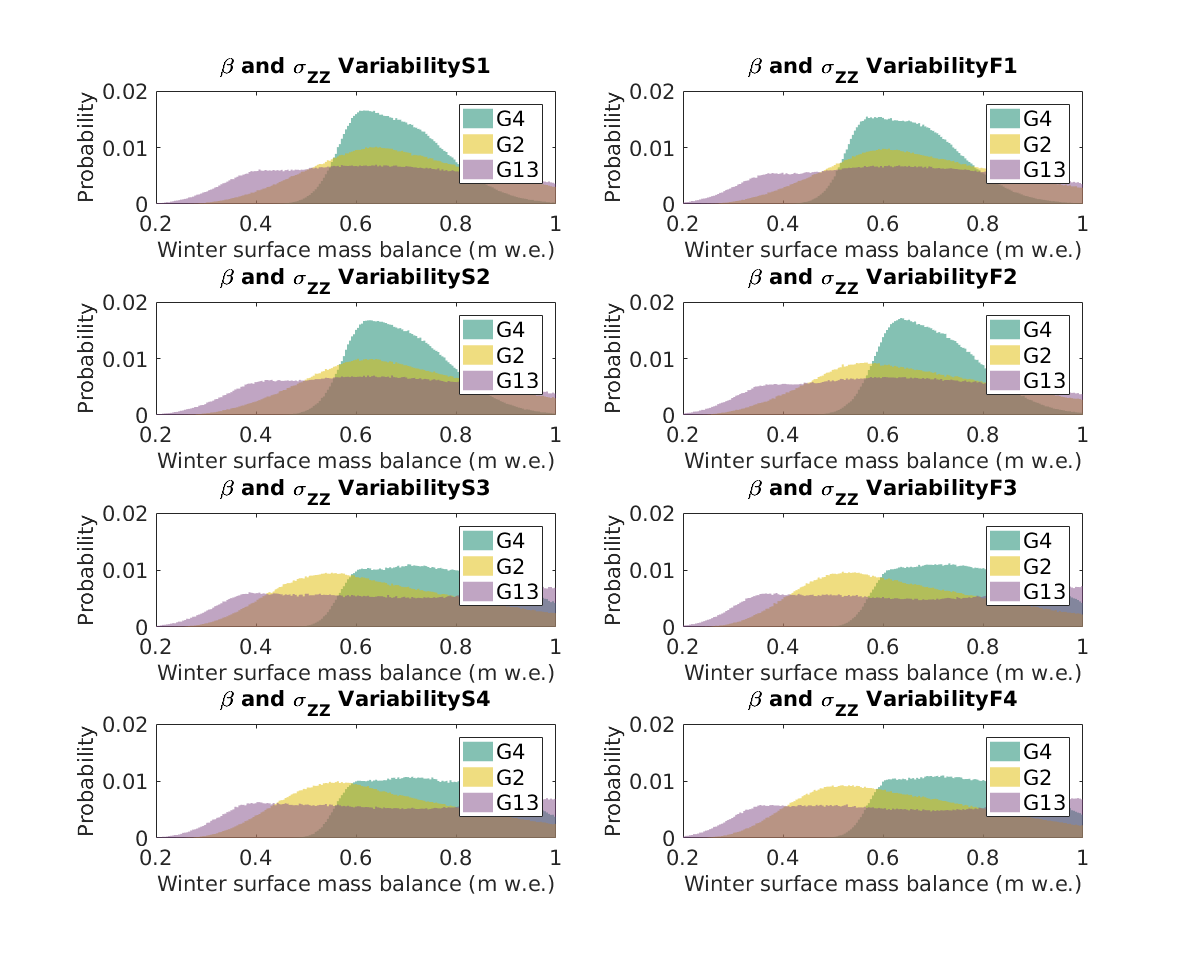
\includegraphics[width =1.2\textwidth]{WSMB_DistributionbetaNzz.png}}\\
	\caption{Winter surface mass balance distribution obtained using linear regression for eight density interpolation options when variation due to regression coefficient estimation and SWE measurement ($\beta$ and $\sigma_{ZZ}$) is included. }
	\label{fig:WSMB_DistributionbetaNzz}
\end{figure}


\subsection{Simple kriging WSMB distribution}

\begin{figure}[H]
	\centering
	\makebox[\textwidth][c]{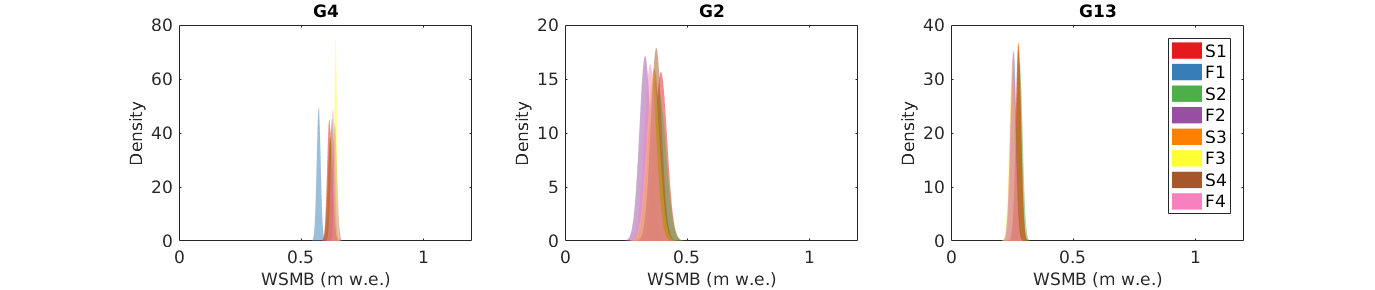
\includegraphics[width=1.2\textwidth]{WSMB_SK_allDensity_zz.png}}\\%
	\makebox[\textwidth][c]{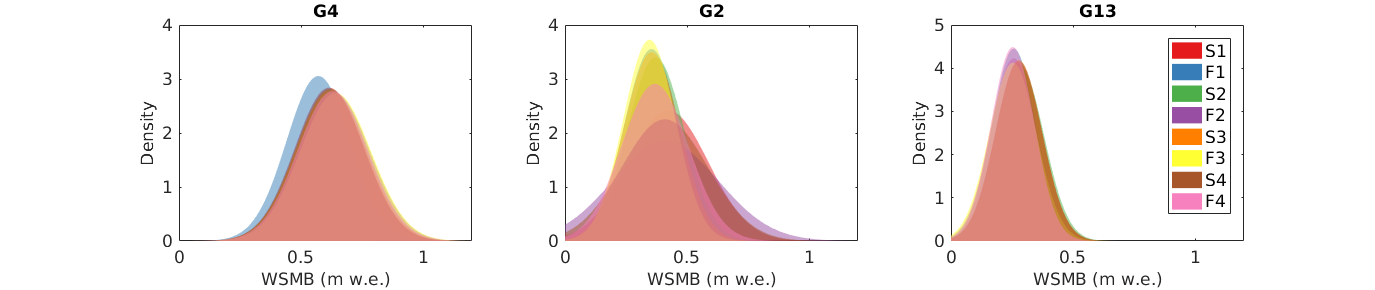
\includegraphics[width=1.2\textwidth]{WSMB_SK_allDensity_beta.png}}\\%
	\makebox[\textwidth][c]{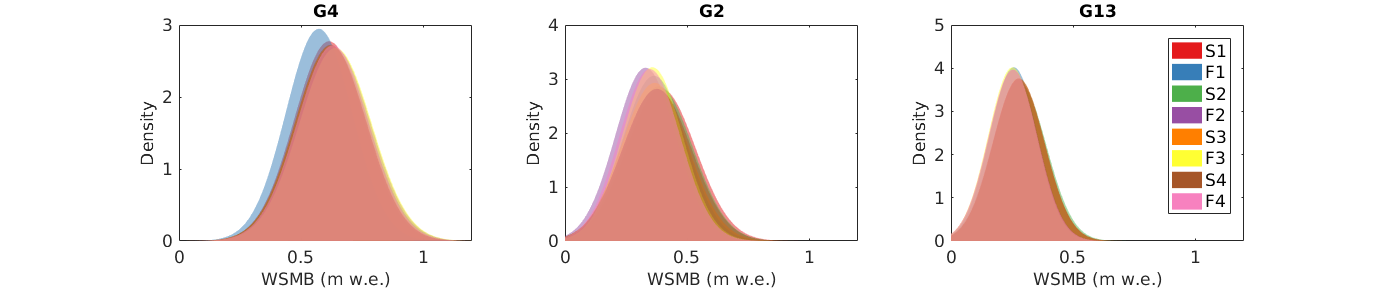
\includegraphics[width=1.2\textwidth]{WSMB_SK_allDensity_betaNzz.png}}%
	\caption{Distribution of winter surface mass balance (WSMB) obtained using simple kriging. (Top) WSMB values obtained from a Monte Carlo sampling of normally distributed SWE variation (obtained from zigzag measurements) about the local SWE value. (Middle) WSMB values obtained from a Monte Carlo sampling of normally distributed regression coefficients. (Bottom) WSMB values obtained using both SWE variability and regression coefficient variability. Eight different density interpolation methods are used to obtain SWE values used in the regression.}
	\label{fig:WSMB_allDensity}
\end{figure}


\begin{figure}[H]
	\centering
	\makebox[\textwidth][c]{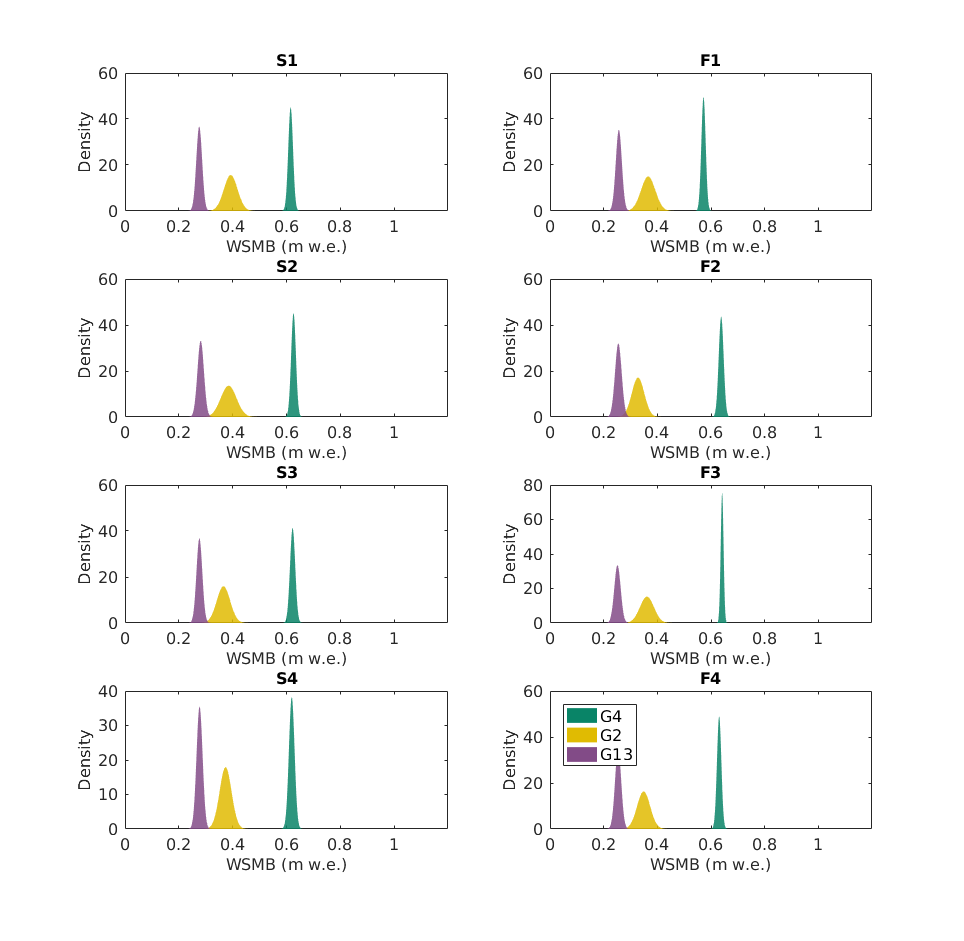
\includegraphics[width =1.2\textwidth]{WSMB_Distribution_SK_zz.png}}\\
	\caption{Winter surface mass balance distribution obtained using simple kriging for eight density interpolation options when variation due to SWE measurement ( $\sigma_{ZZ}$) is included. }
	\label{fig:WSMB_Distributionzz}
\end{figure}
\begin{figure}[H]
	\centering
	\makebox[\textwidth][c]{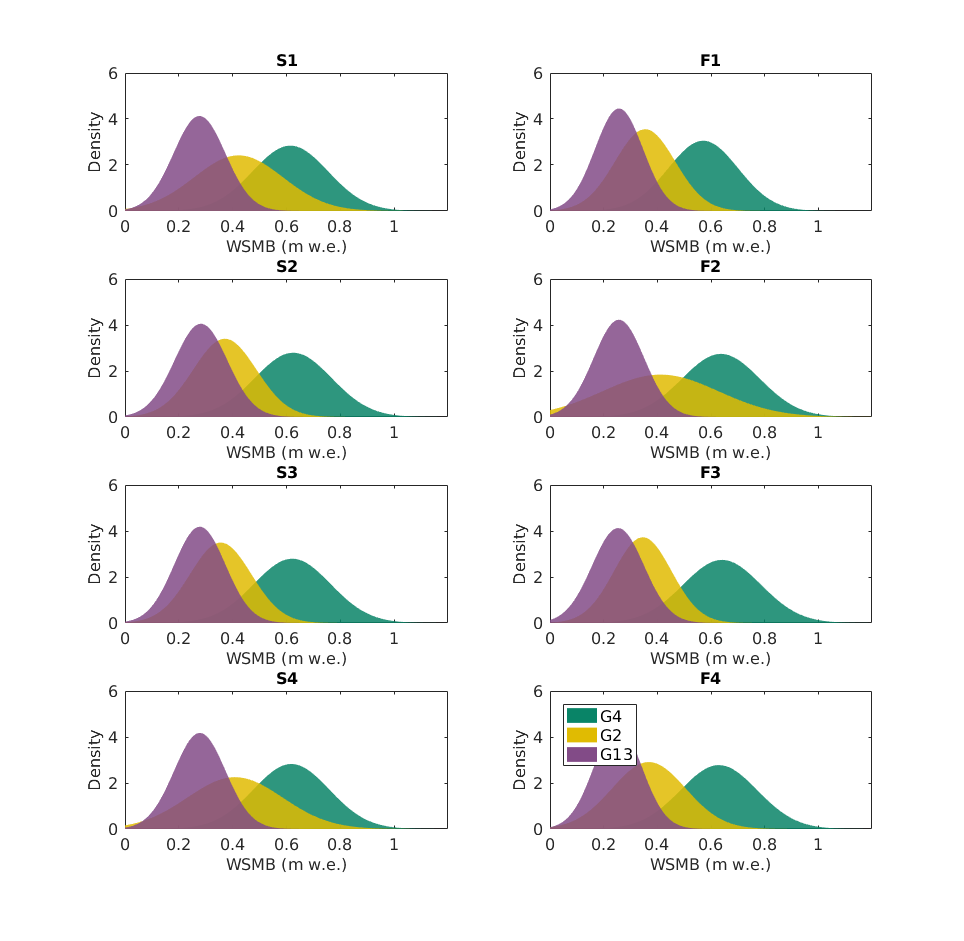
\includegraphics[width =1.2\textwidth]{WSMB_Distribution_SK_beta.png}}\\
	\caption{Winter surface mass balance distribution obtained using simple kriging for eight density interpolation options when variation due to regression coefficient estimation ( $\beta$) is included. }
	\label{fig:WSMB_Distributionbeta}
\end{figure}
\begin{figure}[H]
	\centering
	\makebox[\textwidth][c]{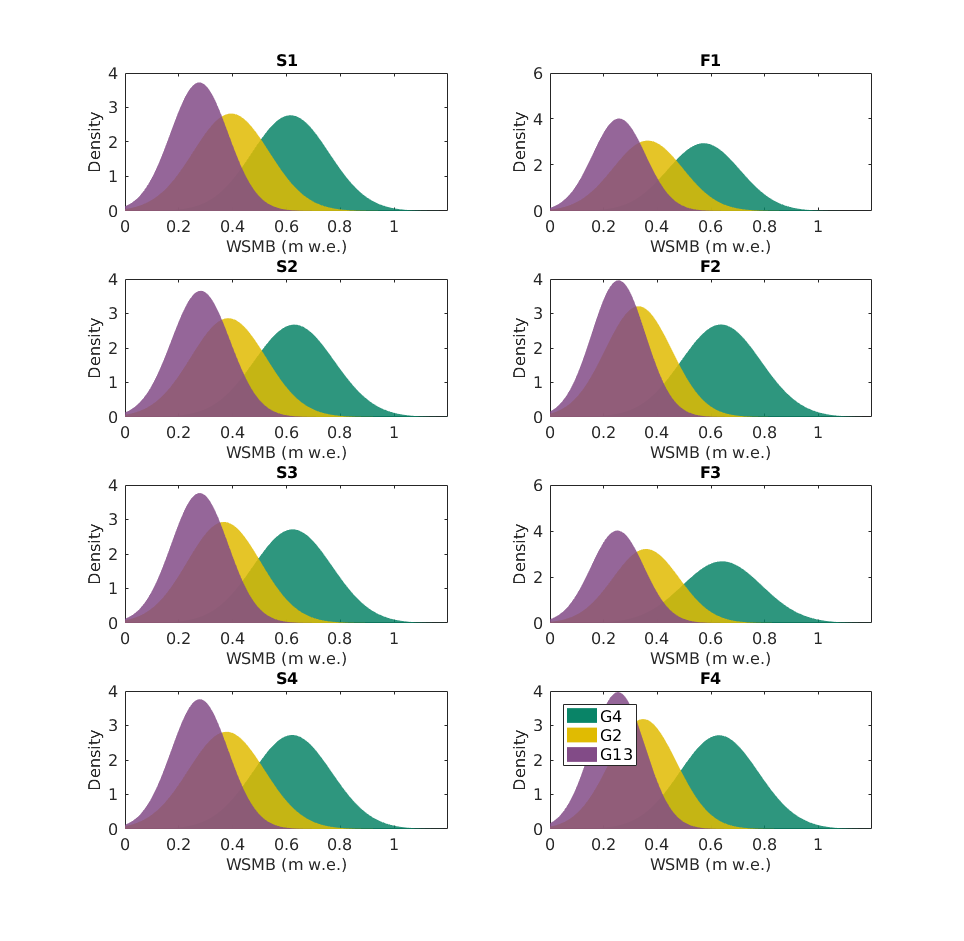
\includegraphics[width =1.2\textwidth]{WSMB_Distribution_SK_betaNzz.png}}\\
	\caption{Winter surface mass balance distribution obtained using simple kriging for eight density interpolation options when variation due to regression coefficient estimation and SWE measurement ($\beta$ and $\sigma_{ZZ}$) is included. }
	\label{fig:WSMB_DistributionbetaNzz}
\end{figure}

\end{document} 